\section{Design Requirements \& Hardware Implementation} \label{sec:hardware}\label{sec:design_requirements}

\subsection{Purpose \& Deployment Procedure}
%The goal with the CALibration source Insertion System (CALIS) is to study and calibrate the detector response of the \tpc\ and the \lsv\ as well as the detection efficiency of internal neutrons interacting in the \tpc\ and \lsv\ using radioactive gamma and neutron sources. 

The CALibration Insertion System (CALIS) deploys radioactive gamma and neutron sources inside the LSV to study and calibrate the \tpc\ and the \lsv\ detector response and neutron detection efficiency. For \tpc\ calibration the radioactive source has to be positioned in immediate contact with the cryostat, in order to minimize rate losses through absorption. This is especially important for low energy sources such as $^{57}$Co (122 keV). 

As shown in Fig.~\ref{fig:DeploymentDevice}, right, there is a gap between the 32 cm wide cryostat and the organ pipe, whose central axis is 80 cm away from the TPC's vertical z-axis. This gap precludes a single cable solution deployed from within a glove box as used in several other scintillator experiments \cite{Banks:2014hra, Huang:2013uxa}. %\cite{KamLAND-MiniCal, DayaBay_zaxis}.
Instead our apparatus consists of an enclosure which has been installed in CRH and the deployment device featuring an articulation mechanism. Inside the enclosure the deployment device is mounted through two stainless steel cables wound around cable spools. The deployment device contains the mechanical support structure for the source arm, which holds the calibration source at its tip and the gear to articulate it. Focusing just on the mechanics, i.e.~after successful source insertion, a deployment consists of three steps as illustrated in Fig.~\ref{fig:DeploymentDevice}:
\begin{enumerate}
\renewcommand{\theenumi}{\Alph{enumi}} %http://tex.stackexchange.com/questions/2291/how-do-i-change-the-enumerate-list-format-to-use-letters-instead-of-the-defaul
\item Lowering the deployment device into the \lsv with the source arm dearticulated,
\item articulation of the source arm to horizontal, while the arm is still rotated away from the cryostat in the $xy$-plane and
\item the rotation of the device in the $xy$-plane to bring the calibation source into contact with the cryostat.
\end{enumerate}
In order to return the deployment device from the \lsv\ the sequence and every step is inversed.

\begin{figure}[htbp]
 \centering
%\includegraphics[height=0.7\textheight,clip=true]{Figures/DeploymentDevice}
%\includegraphics[height=0.4\textheight]{Figures/CALIS_sideview_Cary.jpg}
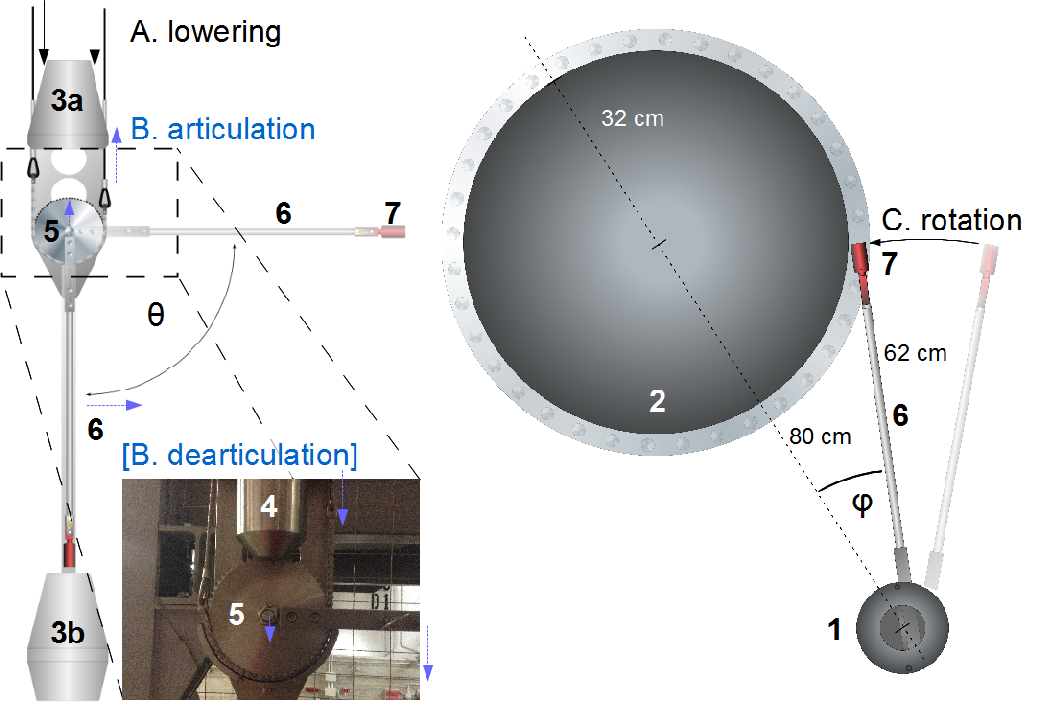
\includegraphics[width=\textwidth]{Figures/DeploymentDevice_XY_view2} %0.65\textwidth would work
  \caption{A side view \textit{(left)} and top view \textit{(right)} of the deployment device (1) next to the \tpc's cryostat (2) is shown. The deployment device features cones at the top and bottom (3a,b), weights (4), an articulation gear (5) and the source arm (6) with the source holder (7) at its tip. A deployment into the \lsv\ involves three steps: \textit{A. lowering} the device into the \lsv\ with the source arm dearticulated, \textcolor{blue}{\textit{B. articulation} of the source arm to horizontal, while the arm is still rotated away in the $xy$-plane and} \textit{C. rotation} of the device to have the source in contact with the cryostat. (In order to distinguish the '\textcolor{blue}{articulation}' from the 'lowering', arrows and captions related to articulation are highlighted in blue in the figure.) Articulation can be set to any angle $\theta$ between 0$^{\circ}$ and 90$^{\circ}$, with horizontal articulation corresponding to 90$^{\circ}$ and dearticulation to 0$^{\circ}$. During calibration campaigns by default the arm length was 62 cm and the source arm was articulated to horizontal. The cryostat's outer radius is 32 cm, the organ pipe is off from the TPC's vertical z-axis by 80 cm.\label{fig:DeploymentDevice}}
\end{figure} 


\subsection{Deployment \& Articulation Mechanism}\label{sec:DeploymentArticulation}
%This way the gap between the organ pipe and cryostat is bridged. The articulation mechanism requires two cables and  

%The deployment and articulation modes are illustrated both in Figs.~\ref{fig:DeploymentDevice} and \ref{fig:CALISMechanism}. 
As shown in Fig.~\ref{fig:CALISMechanism}, the stepper motor moves both cable spools concurrently and thereby sends the deployment device into the \lsv. An absolute encoder provides its current position, even in the absence of power. The stepper motor is controlled via a simple graphical LabVIEW interface, run on a dedicated laptop, in which the current $z$-position is shown and a target $z$-position can be provided by the operator. $Z$-positions are given in motor step counts, an arbitrary unit which has been calibrated outside CRH in meters (Fig.~\ref{fig:z_test}), as well as relative to the TPC using \tdrift\ distributions from calibration data (Sec.~\ref{sec:SourcePosition}). \label{sec:Nonlinearity:MotorStepCounts}
The non-linearity between motor steps and cable length shown in Fig.~\ref{fig:z_test} arises as follows: As the cables wind around their spools, the winding radius changes, increasing as the deployment device is lifted and decreasing as it is lowered. A motor step count corresponds to a fixed angular distance \textit{d$\theta$}, yet the amount of cable deployed during this motor step is \textit{winding radius $\cdot$ d$\theta$}. As the winding radius changes as a function of $z$-position, the fraction of deployed cable per motor step count changes.

\begin{figure}[htbp]
 \centering
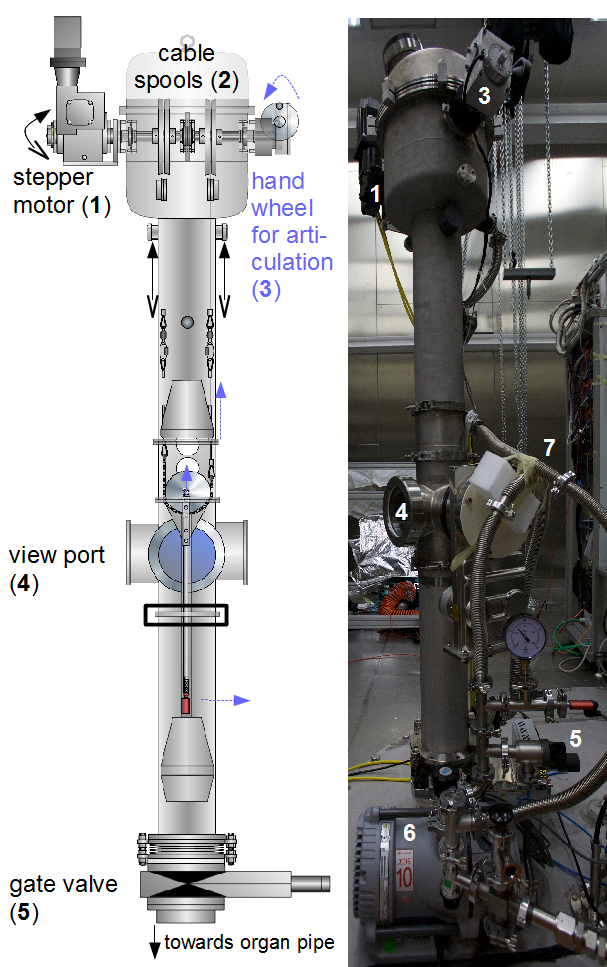
\includegraphics[width=0.8\textwidth]{Figures/CALIS_overview.png}
 %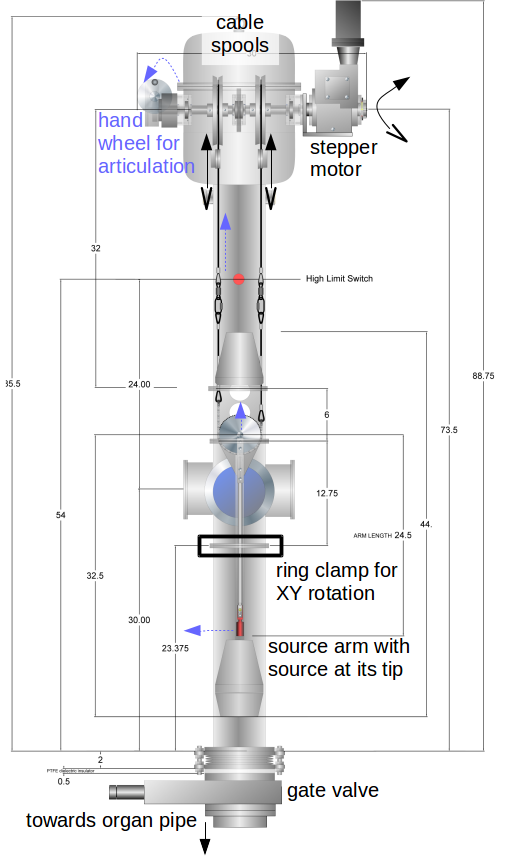
\includegraphics[width=0.68\textwidth]{Figures/CALISDimensions.png}
 %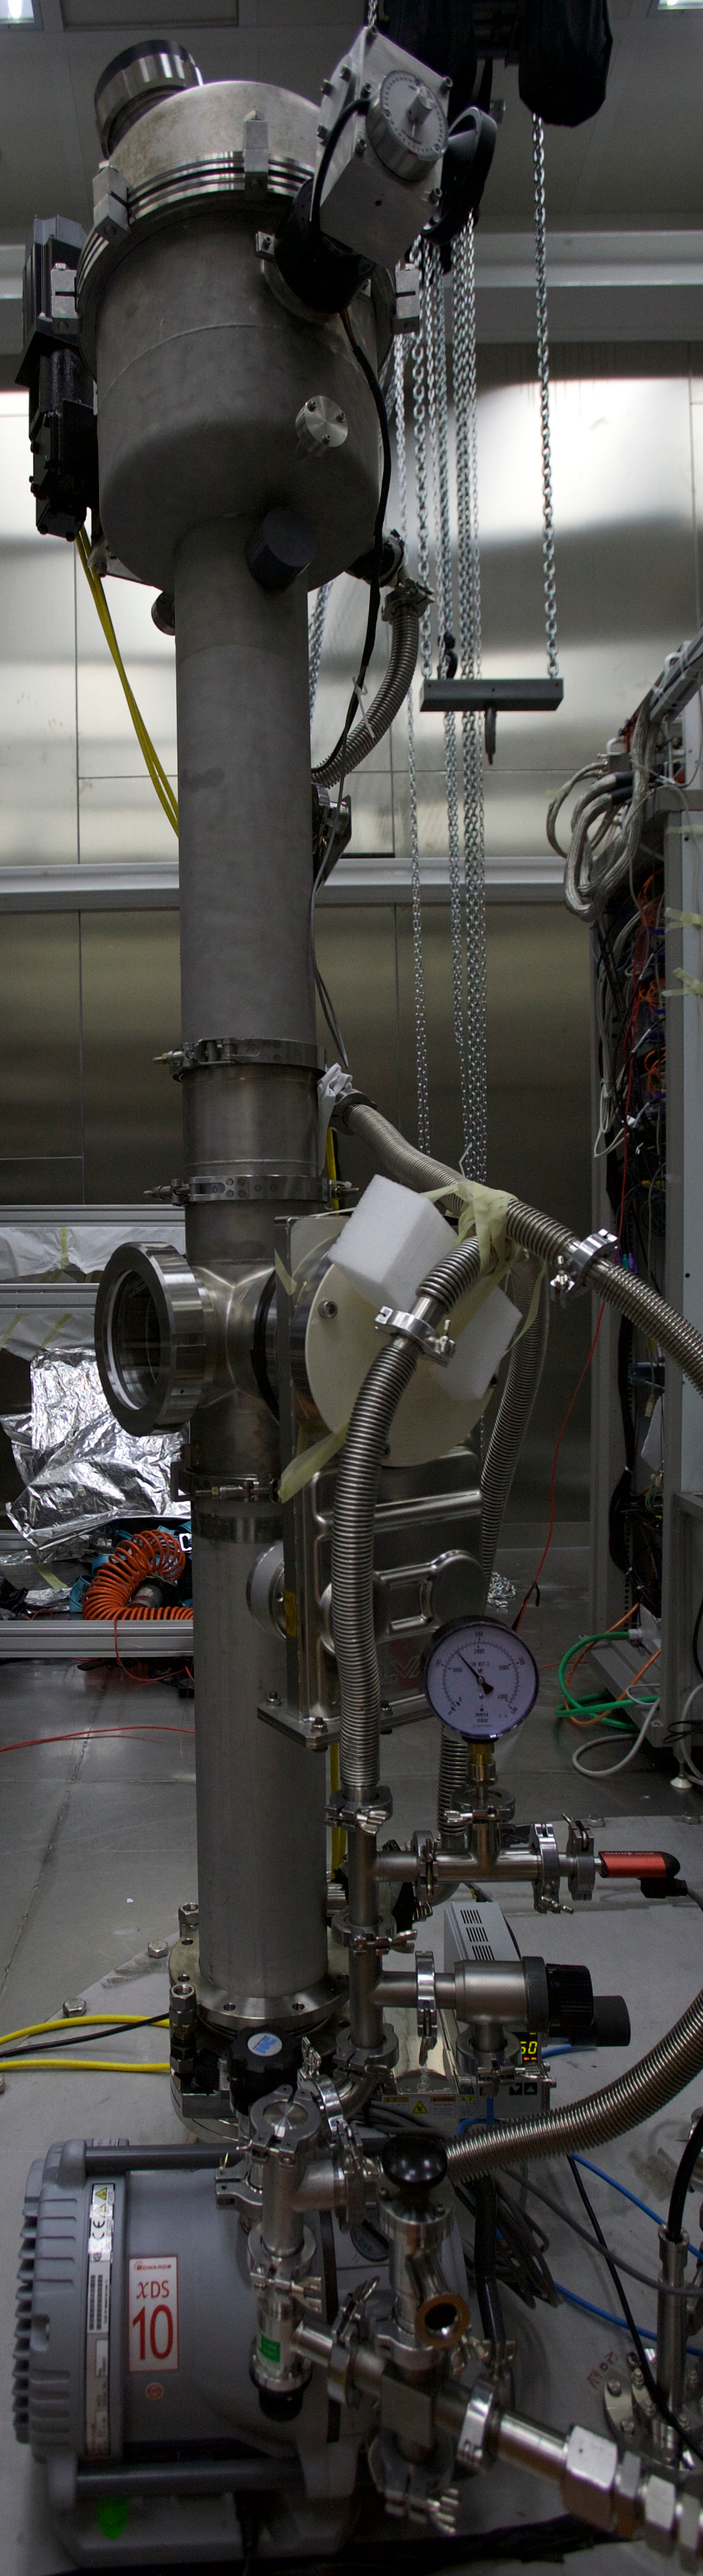
\includegraphics[width=0.30\textwidth]{Figures/CALIS_overview_IMG_3763.jpg}
 \caption{Mechanical drawing of CALIS showing the housing and the deployment device in its home position next to a photo of CALIS as installed inside the clean room CRH. The total height is approx.~240 cm including the gate valve. The 'lowering' and 'articulation' modes of operation are illustrated, the latter is highlighted in blue to distinguish it from the former: In order to move the deployment device down into the \lsv\ (or back up), the stepper motor moves both cable spools (2) concurrently. \textcolor{blue}{In order to articulate, the articulation wheel (3) is rotated manually, which affects only the right spool, thereby shortening the right cable with respect to the left cable, engaging the gear, articulating the arm and lifting the pivot center.} The amount of lifting and the amount of rotations until a horizontal articulation is reached has been calibrated prior to installation in CRH (Sec.~\ref{sec:Testing}). Through the view port (4) the source arm is manipulated. The ring clamp (5) is used for rotations in the $xy$-plane and the tripod (6) has been used for vertical alignment of CALIS wrt.~the organ pipe, which is closed by the gate valve (7). 
In the photograph the vacuum pump (8) and tubing (9) are shown, which are part of the evacuation and purging system (Sec.~\ref{sec:EvacPurge}). \label{fig:CALISDimensions}\label{fig:CALISMechanism}\label{fig:gearDrawing}\label{fig:flushing_purging}
}
\end{figure}

\begin{figure}[htbp]
 \centering
 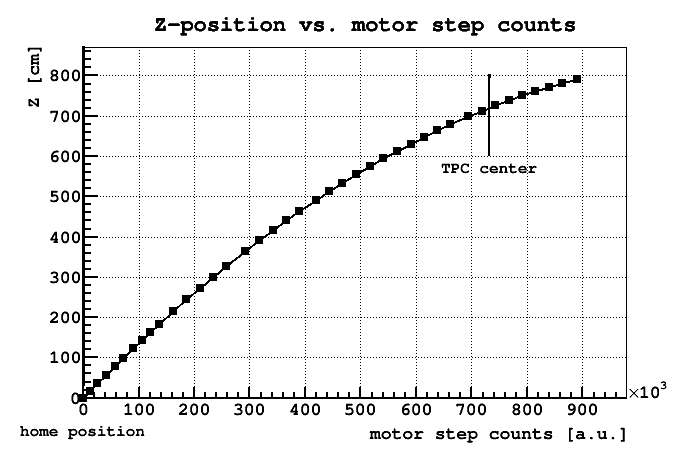
\includegraphics[width=0.8\textwidth]{Figures/MSC_Z}
%at 0.6 textwidth the plot is on a separate page
 \caption{Plot of the deployment device's $z$-position versus motor step counts. The non-linear correspondence between number of steps and cable length deployed arises as follows: As the cables wind around their spools, the winding radius changes, increasing as the deployment device is lifted and decreasing as it is lowered. A motor step count corresponds to a fixed angular distance \textit{d$\theta$}, yet the amount of cable deployed during this motor step is \textit{winding radius $\cdot$ d$\theta$}. As the winding radius changes as a function of $z$-position, the fraction of deployed cable per motor step count changes. The home position is at 0, the TPC center is reached after more than 7 m of travel into the \lsv, the maximum depth is reached at nearly 8 m.}
 \label{fig:z_test}
\end{figure}


Source arm articulation is done manually via the articulation wheel. This affects only the cable spool close to the articulation wheel, the right one in Fig.~\ref{fig:CALISMechanism}, thereby shortening the right cable with respect to the left cable and engaging the gear through a chain. As a result the source arm is articulated and the pivot center is lifted. The non-linearity between motor steps and cable length affects also the amount of rotation required by the hand wheel for horizontal source arm articulation. Degrees on the articulation wheel corresponding to a horizontal articulation have been calibrated as a function of $z$-position prior to installation in CRH.

Articulation and a movement in $z$-direction are mutually exclusive since arm articulation leads to more cable wound up on the spool close to the articulation wheel with respect to the other. If then, in $z$-movement mode, both spools would be rotated simultaneously with the same angular speed, the cable close to the articulation wheel would wind up faster than the other, leading to a build up of difference in cable length and the deployment device would only be hanging on one cable. In order to avoid an imbalanced $z$-movement, the arm has to be dearticulated fully before a change in $z$-position can be initiated. This is enforced by an electric switch preventing $z$-movement, which is disengaged only when the source arm is fully dearticulated (i.e.~hanging vertically). 

\subsubsection*{Deployment Device}
As shown in Fig.~\ref{fig:DeploymentDevice} the device is equipped with tapered cones on its top and bottom, ensuring that the ends do not get snagged on inner edges as it moves down and up, such as when reentering the organ pipe from the inside of the \lsv\ while on its way back to its home position inside the CALIS enclosure. It is attached to the housing by two cables. Swivel hooks are employed in the attachment of the cables to the deployment device allowing them to move freely and not get tangled. 
There are two weights built into the device, one cylindrical in the conical cap above the rotation gear mechanism and one inside the cone at the device's bottom end. Both help to minimize any lateral motion or oscillations during deployment, articulation and dearticulation. They also ensure smooth motion of the deployment device into the organ pipe and back to the home position.

%Discussion:
% why no permanent tube?
% To complement studies of nuclear recoils with neutron sources ($^{241}$Am$^{9}$Be and $^{241}$Am$^{13}$C), it is planned to deploy a 

\subsection{CALIS Enclosure \& Scintillator}

Besides providing mechanical support for the deployment device via the cable spools, the CALIS enclosure is an important interface between the radon-free clean room CRH and the \lsv, through which sources are exchanged. 
The enclosure protects the liquid scintillator (LS) and prevents human contact with any traces of harmful LS vapor (Fig.~\ref{fig:CALISMechanism}). It plays the same role as a glove box for similar calibration systems, yet with a narrower foot print inside CRH. The liquid scintillator is a mixture of pseudocumene (PC) and trimethyl borate (TMB) with the wavelength shifter 2,5-diphenyloxazole (PPO) \cite{Agnes:2015qyz}.\footnote{The concentration of TMB and PPO have been varied during campaigns (see Sec.~\ref{sec:CalibCampaigns}).} %\cite{vetoPaper}. 
It must not be exposed to oxygen or water that is present in normal clean room air. Contamination of the LS with $^{222}$Rn and its long-lived radioactive daughters has to be avoided, as well. 

Going up from the gate valve on which CALIS has been installed, there is a teflon disk that can electrically isolate CALIS from ground, even though during normal operations the CALIS housing is connected to ground. A tripod with a bellow has been used to vertically align the enclosure right after installation on the gate valve. The bellow is connected to a 59.4 cm long cylindrical stainless steel enclosure pipe. It has the same diameter as the organ pipe (15 cm) and is connected to the view port by a ring clamp, which plays a critical role for rotations in the $xy$-plane (see Sec.~\ref{sec:XYrotation}). The view port can be opened for handling the source arm and exchanging calibration sources. Everything above the ring clamp forms the upper assembly. It features a stainless steel cylindrical enclosure housing the cable drive mechanism, including the cable spools, the stepper motor and the articulation mechanism already described in Sec.~\ref{sec:DeploymentArticulation}. 

\subsubsection*{Vacuum evacuation (flushing) and nitrogen purging system}\label{sec:EvacPurge}
One of this system's most important safety features is making sure that TMB and PC residue on the deployment device are extracted from CALIS and vented prior to opening the view port to access the source arm. This is important for safe working conditions inside CRH as well as for the scintillator and its radiopurity. 

After the source arm insertion and view port closure, the inside of the CALIS housing is filled with normal air that is damaging to the scintillator. A sequence of evacuations and nitrogen purges reduces the fraction of normal air and its contaminants in the air-N$_2$ mixture to negligible levels. Only after this sequence is finalized, the gate valve is opened and the deployment device is introduced into the \lsv. Evacuation is achieved with a vacuum pump and the exhaust air is removed through dedicated vent lines (Fig.~\ref{fig:flushing_purging}).

At the end of a calibration campaign, after the deployment device has returned to its home position inside the enclosure and the gate valve has been closed, scintillator vapor, and in particular TMB, has to be removed prior to opening the view port. Again a sequence of evacuation and nitrogen purges is employed. By lowering the pressure inside of CALIS below the TMB and PC vapor pressure, the scintillator evaporates and is removed through the vacuum pump vent line. Once pressure inside the housing stays consistently below the vapor pressure of TMB, all scintillator has been removed and the view port can be opened to access the source arm.
 
\subsubsection*{Material Compatibility}
All materials coming in contact with the scintillator veto are made of stainless steel or teflon, except for the sealing o-rings which are made of viton. All three materials are certified for contact with all scintillator components including TMB and PC.

\subsection{Source Arms and Source Holder}
A source arm and source holder are attached to an articulation gear. Different arm lengths have been prepared, with a maximum arm length of 62 cm as measured from the pivot point of the rotation gear to the source holder's tip. The radioactive source is housed inside the source holder (Fig.~\ref{fig:SourceHolder}). During deployment it is pressed to the tip and held in place via a spring. The source holder is sealed such that no liquid scintillator can enter during deployment. This has also been verified during each source extraction and no liquid traces have been found inside.
%already mentioned elsewhere: This arm length allows the source to be placed in immediate contact with the cryostat (Fig.~\ref{fig:CALIS_photos}, right), since the organ pipe's center axis is 80 cm from the TPC center and the cryostat has an outer radius of 32 cm. The 62 cm arm was used by default for deployments in past calibration campaigns (Sec.~\ref{sec:CalibCampaigns}).

\begin{figure}[htbp]
 \centering
  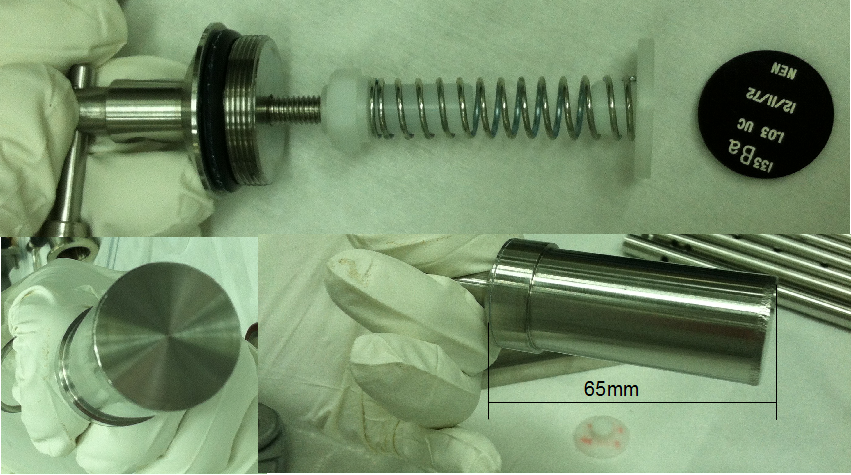
\includegraphics[width=0.7\textwidth]{Figures/SourceHolder.png}
  \caption{The source holder that connects to an arm and to the articulation gear of the deployment device. The source, here a $^{133}$Ba source, is pressed to the tip of the source holder via a spring.}
  \label{fig:SourceHolder}
\end{figure}